%!TEX root = ../thesis.tex
%*******************************************************************************
%****************************** Fourth Chapter *********************************
%*******************************************************************************

\chapter{Colocalisation of immune infiltrates and spatial statistics of immune cell-tumour-stroma interaction}

\ifpdf
    \graphicspath{{Chapter4/Figs/Raster/}{Chapter4/Figs/PDF/}{Chapter4/Figs/}}
\else
    \graphicspath{{Chapter4/Figs/Vector/}{Chapter4/Figs/}}
\fi


\section[Introduction]{Introduction}
Having explored the tissue structure and its relation to CD8 and FOXP3 infiltrate. I found that a measure of surface area to volume ratio was correlated with quantity of FOXP3 infiltrate. This implies that on some level the structural layout of a tissue is related to the amount of contact of immune cells with the epithelium.

As mentioned in the introduction, some methods of immune analysis are capable of measuring many more markers on a single section than standard IHC and IF. IMC is one of the best of such methods, allowing for measuring more than 20 markers on a single tissue section by conjugating antibodies with metal isotopes. This method allowed me to view additional markers for microenvironmental features such as collagen and hypoxia alongside a panel of immune markers that included the ones that had been investigated in previous chapters. In order to investigate the micro-environment in both epithelium and the tumour-adjacent stroma I used the BriTROC and ICON7 cohorts to investigate this.

The 

\subsection{History of the project and roles}
Sarwah Al-Khalidi originally intended to create an IMC panel for immune markers alone, I worked with SAK to include collagen in order to both better delineate stroma tissues from epithelium and investigate the structure of collagen and its interaction with immune cells. Sarwah Al-Khalidi (SAK) carried out the panel optimization and staining on the BriTROC cohort. I arranged for Fatime Cosaj(FC) to carry out the staining with the same panel on the ICON7 cohort using the same protocols as optimized by SAK. I arranged for Richard Grenfell (RG) of the Institute core to carry out the imaging of the stained ICON7 slides on the same machine as the BRITROC cohort had been done.

From the markers included in the IMC panel, the subset of these of markers that I was interested in were;
\begin{itemize}
\item \textbf{CD8, CD68, CD45RO, FOXP3} - Key immune cell populations for comparison with other datasets
\item \textbf{CK7, Collagen1} - Key structural markers, gold standards for comparison of epithelial structure and quantity with other datasets
\item \textbf{CA9} - Hypoxia marker to investigate the relationship between tissue structure and hypoxia
\item \textbf{Ki-67} - Proliferation marker to investigate the relationship between tissue structure and proliferation \end{itemize}

\begin{figure}
    \centering
    \includegraphics{}
    \caption{Visual abstract for this chapter. IMC images are processed and collagen channels as well as multi-immune channels are cleaned and then analysed for structural and spatial features.}
    \label{fig:ch5_visualabstract}
\end{figure}

\section[Methodology]{Methodology}
\subsection{Cohort Summary}
\subsubsection{BriTROC} Samples were collected previous to this PhD under the British Translational Research Ovarian Cancer Collaborative (BriTROC), a non-randomised prospective study enrolling patients with recurrent HGSOC\cite{}.  Figure \ref{fig:BriTROC_remark} shows the REMARK diagram for this cohort. A total of 446 diagnostic samples were collected from 276 patient with relapsed HGSOC. 247 samples from 172 patients had enough material to generate a tissue microarray (TMA) for immunohistochemistry staining. Three 1mm cores from the tumour area of each sample were marked on H&E-stained slides by a pathologist, and used by Darren Ennis to make a tissue microarray (TMA) of the samples.
\begin{figure}
    \centering
    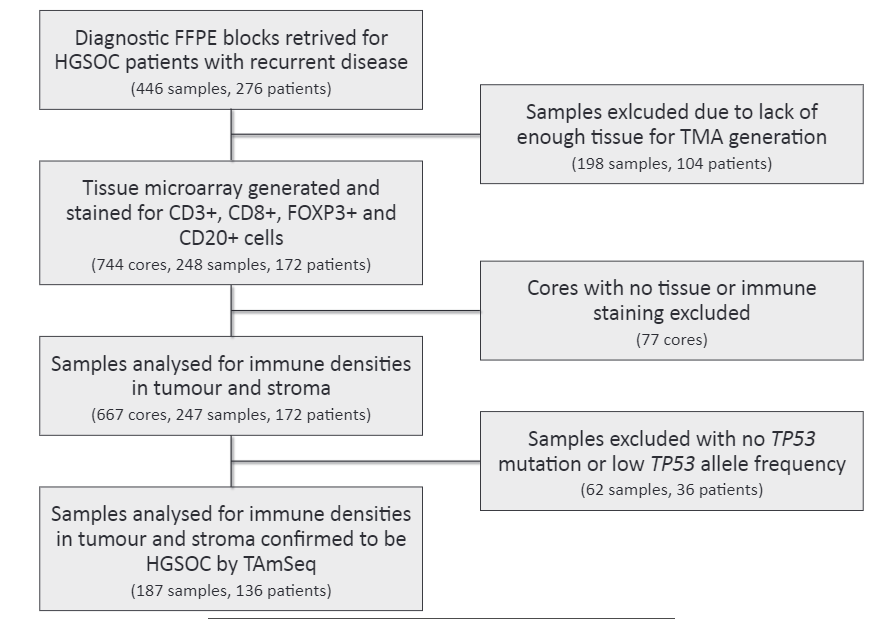
\includegraphics{Chapter4/figs/remark_britroc.png}
    \caption{REMARK diagram for the BriTROC cohort.}
    \label{fig:BriTROC_remark}
\end{figure}


\subsubsection{ICON7}
ICON7 was an international, phase 3, open-label, randomised trial undertaken at 263 centres in 11 countries across Europe, Canada, Australia and New Zealand. Eligible adult women with newly diagnosed ovarian cancer that was either high-risk early-stage disease (International Federation of Gynecology and Obstetrics [FIGO] stage I–IIa, grade 3 or clear cell histology) or more advanced disease (FIGO stage IIb–IV), with an Eastern Cooperative Oncology Group performance status of 0–2, were enrolled and randomly assigned in a 1:1 ratio to standard chemotherapy (six 3-weekly cycles of intravenous carboplatin [AUC 5 or 6] and paclitaxel 175 mg/m2 of body surface area) or the same chemotherapy regimen plus bevacizumab 7·5 mg per kg bodyweight intravenously every 3 weeks, given concurrently and continued with up to 12 further 3-weekly cycles of maintenance therapy. Randomisation was done by a minimisation algorithm stratified by FIGO stage, residual disease, interval between surgery and chemotherapy, and Gynecologic Cancer InterGroup group. The primary endpoint was progression-free survival; the study was also powered to detect a difference in overall survival. Analysis was by intention to treat. This trial is registered as an International Standard Randomised Controlled Trial, number ISRCTN91273375\cite{Perren2011Dec, BibEntry2020Jan}. Figure \ref{fig:icon_remark} is a REMARK diagram of samples analysed. TMA prepared by MRC.

ICON7 had cores sampled specifically from Epithelium and adjacent stroma, making it ideal for measurement of the microenvironment and measurement of both tumour and stroma in a single section which had been limited to a subset of the patients in previous cohorts.

\subsection{Immuno Metal Conjugation}
The protocol for IMC staining and imaging was carried out by SAK/FC as described in Section \ref{sec:sarwah_staining}.

\subsection{Marker Panel}
The marker panel is specified in section \ref{table:imc_antibodies} and I worked with SAK to include Collagen in this panel for further investigation alongside the immune populations. 


\subsection{Staining and Imaging}
Staining and imaging of the BriTROC panel was carried out by SA-K. Staining and imaging of the ICON7 TMAs was carried out by Fatime Cosaj(FC) and Richard Grenfell(RG) accordingly.

\subsection{Image Analysis}
Python was used for data cleaning and Halo was used for the subsequent analysis of the IMC data files. Structure analysis of signal in the collagen channel was carried out with Imagej and the GLCM, Orientationj and Directionality plugins. 


\section{Results}

As

Before analysing the interaction between these immune cells and these single populations on single tissue sections, I investigated the characteristics of the BriTROC and ICON7 cohorts are shown.

\subsection{BriTROC summary}
\subsection{ICON7 summary}
There were X patients.


\subsection{Immunofluorescence combined with SHG}
In order to assess multiple immune markers on a slide in combination with SHG I decided to use Immunofluorescence, I worked with Jodi Miller (JM) from the Institute core to create an optimized panel to measure CD8, CD68 and nuclear stains simultaneously as well as being able to image the Collagen in the ~450nm channel. We originally utilized DRAQ5 as a nuclear stain. As shown in Figure \ref{fig:IF_protos} the DRAQ5 successfully stained the nuclei but the FITC and Cy3 channels for the CD8+ and CD68+ marker combinations were not successful on FFPE. This was partly due to large amounts of autofluorescence from the FFPE section as well as overlapping FITC and Cy3 emission spectra meaning signal could not be easily distinguished. DAPI/Cy3/Cy5 staining was very clear and chosen for the rest of the imaging.

\begin{figure}
    \centering
    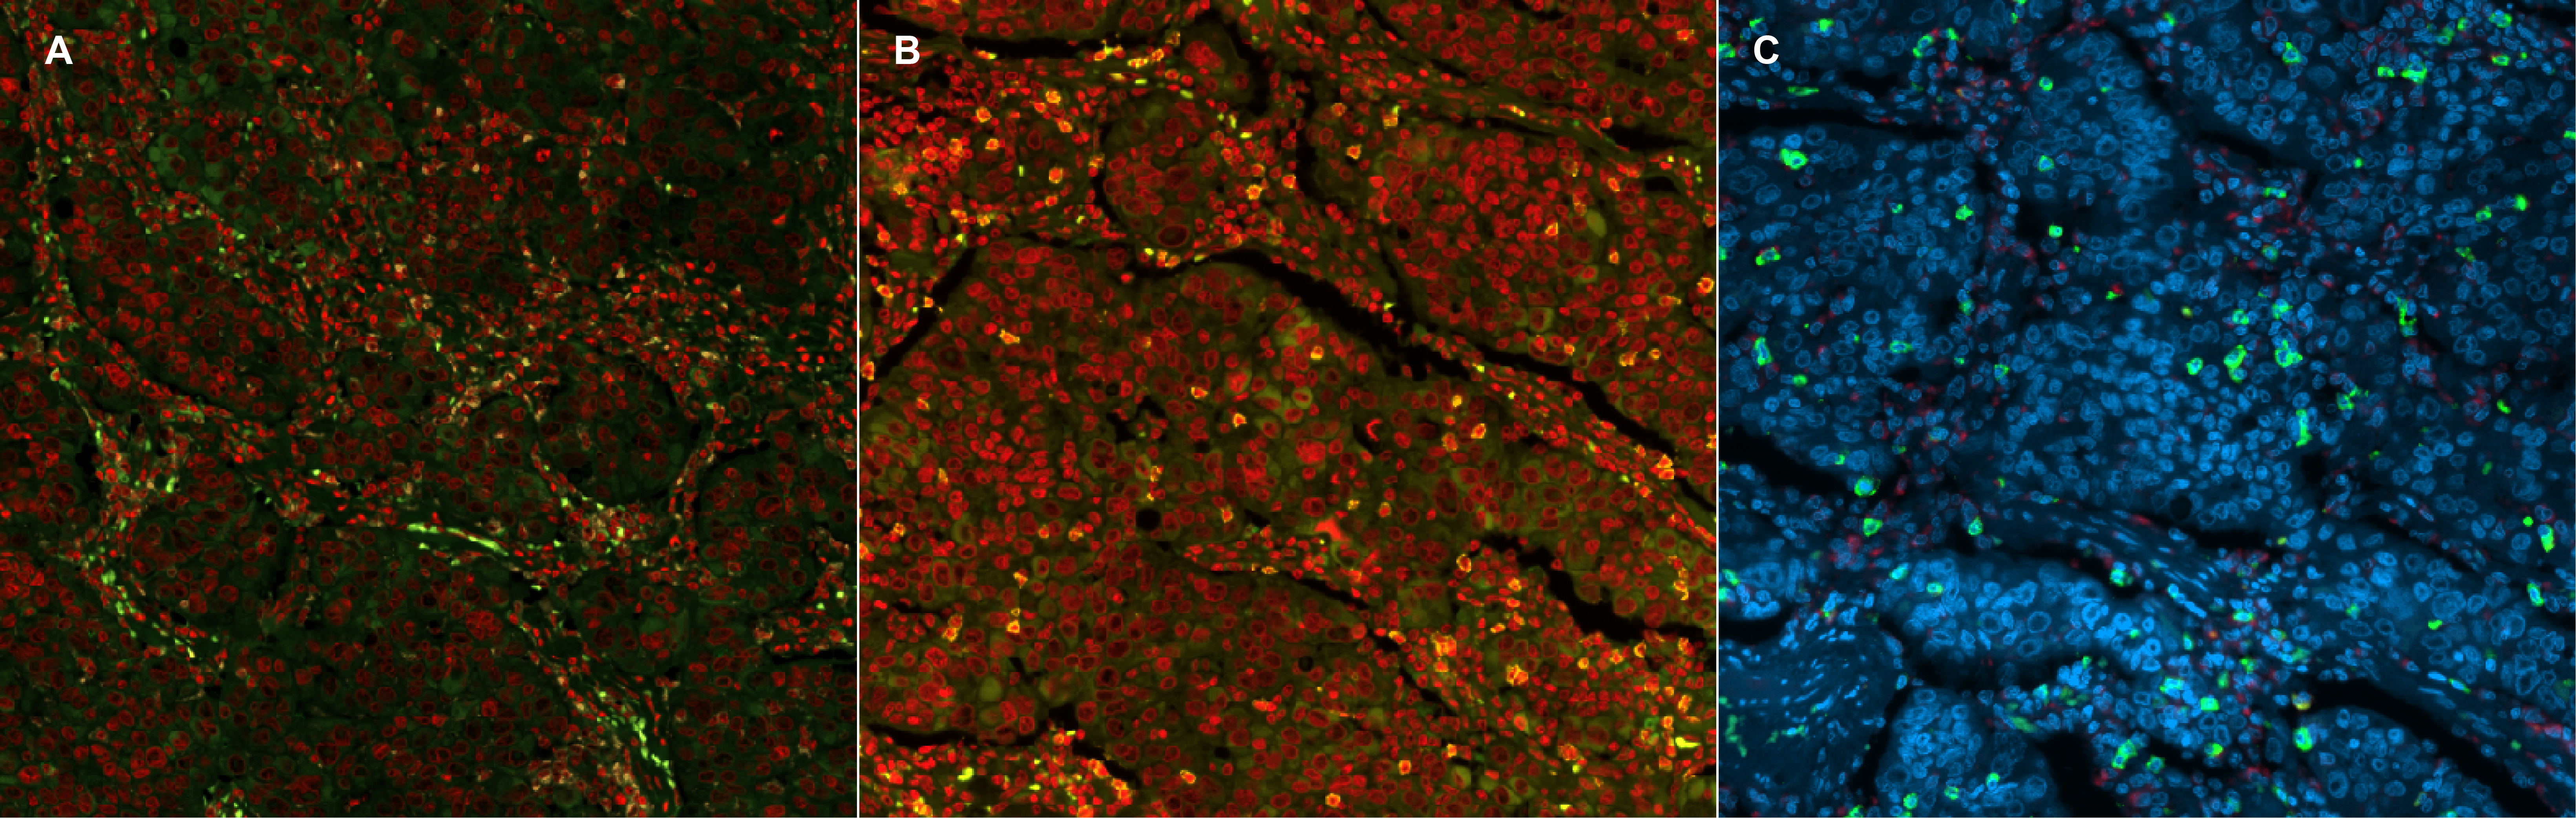
\includegraphics[width=\textwidth]{Chapter4/figs/Thesis-14.png}
    \caption[Images from IF protocols.]{Images from IF protocols. (A) DRAQ5(Cy5), CD8+(FITC), CD68+(Cy3) (B)  DRAQ5(Cy5), CD8+(FITC), CD68+(Cy3)  (C) DAPI, CD8+(Cy3), CD68+(Cy5). CD68+ Macrophages, CD8+ cells and DAPI stained nuclei are very distinct and visible in protocol C.}
    \label{fig:IF_protos}
\end{figure}

Eventually we used DAPI, CD8 and CD68 to obtain a clear image of cells on the section. 

\subsection{IF and SHG combined}
I excited the SHG at a slightly higher wavelength of 920nm in order to raise the wavelength of the emitted signal, this meant that the DAPI cells were not excited too strongly and the image was clear. As shown in figure \ref{fig:SHG_IF}. 
\begin{figure}
    \centering
    \includegraphics[width=0.6\textwidth]{Chapter4/figs/Thesis-13.png}
    \caption[Images measuring IF and SHG signal.]{ DAPI-blue, CD8+(Cy3)-cyan, CD68+(Cy5)-, SHG-red. CD68+ Macrophages, CD8+ cells and DAPI stained nuclei are very distinct and the fibres of collagen are visible in red. Imaged at 40x on SP5.}
    \label{fig:SHG_IF}
\end{figure}

\subsubsection{Collagen structure analysis}
Alongside the use of collagen to classify regions of the tumour and as a marker to identify cells as adjacent to collagen fibres, the collagen channel from IMC can be analysed in the same way as was done for the SHG imaging to analyse the structure and organization of the collagen fibres.

I found that the coherency of the fibres was correlated with. 

\subsection{IMC image analysis}
 IMC images contain hot pixels distributed randomly across the image, in order to clean the data, I carried out hot-spot removal in python using a median filter with a 3x3 pixel area (see Code \ref{script:1}).
 
 I built a classifier in Halo to distinguish epithelial tissue from low density and high density collagen, specified by the intensity of the Collagen1 marker over small areas.
 I then built cell segmentation algorithms based on nuclear DNA marker staining to segment nuclei. I then used the IMC marker panel to classify cells based on their nuclear and cytoplasmic staining. An example of tissue segmentation and cell segmentation and classification of ICON7 and BRITROC image is shown in Figure \ref{fig:IMC_example}.
 
 \begin{figure}
     \centering
     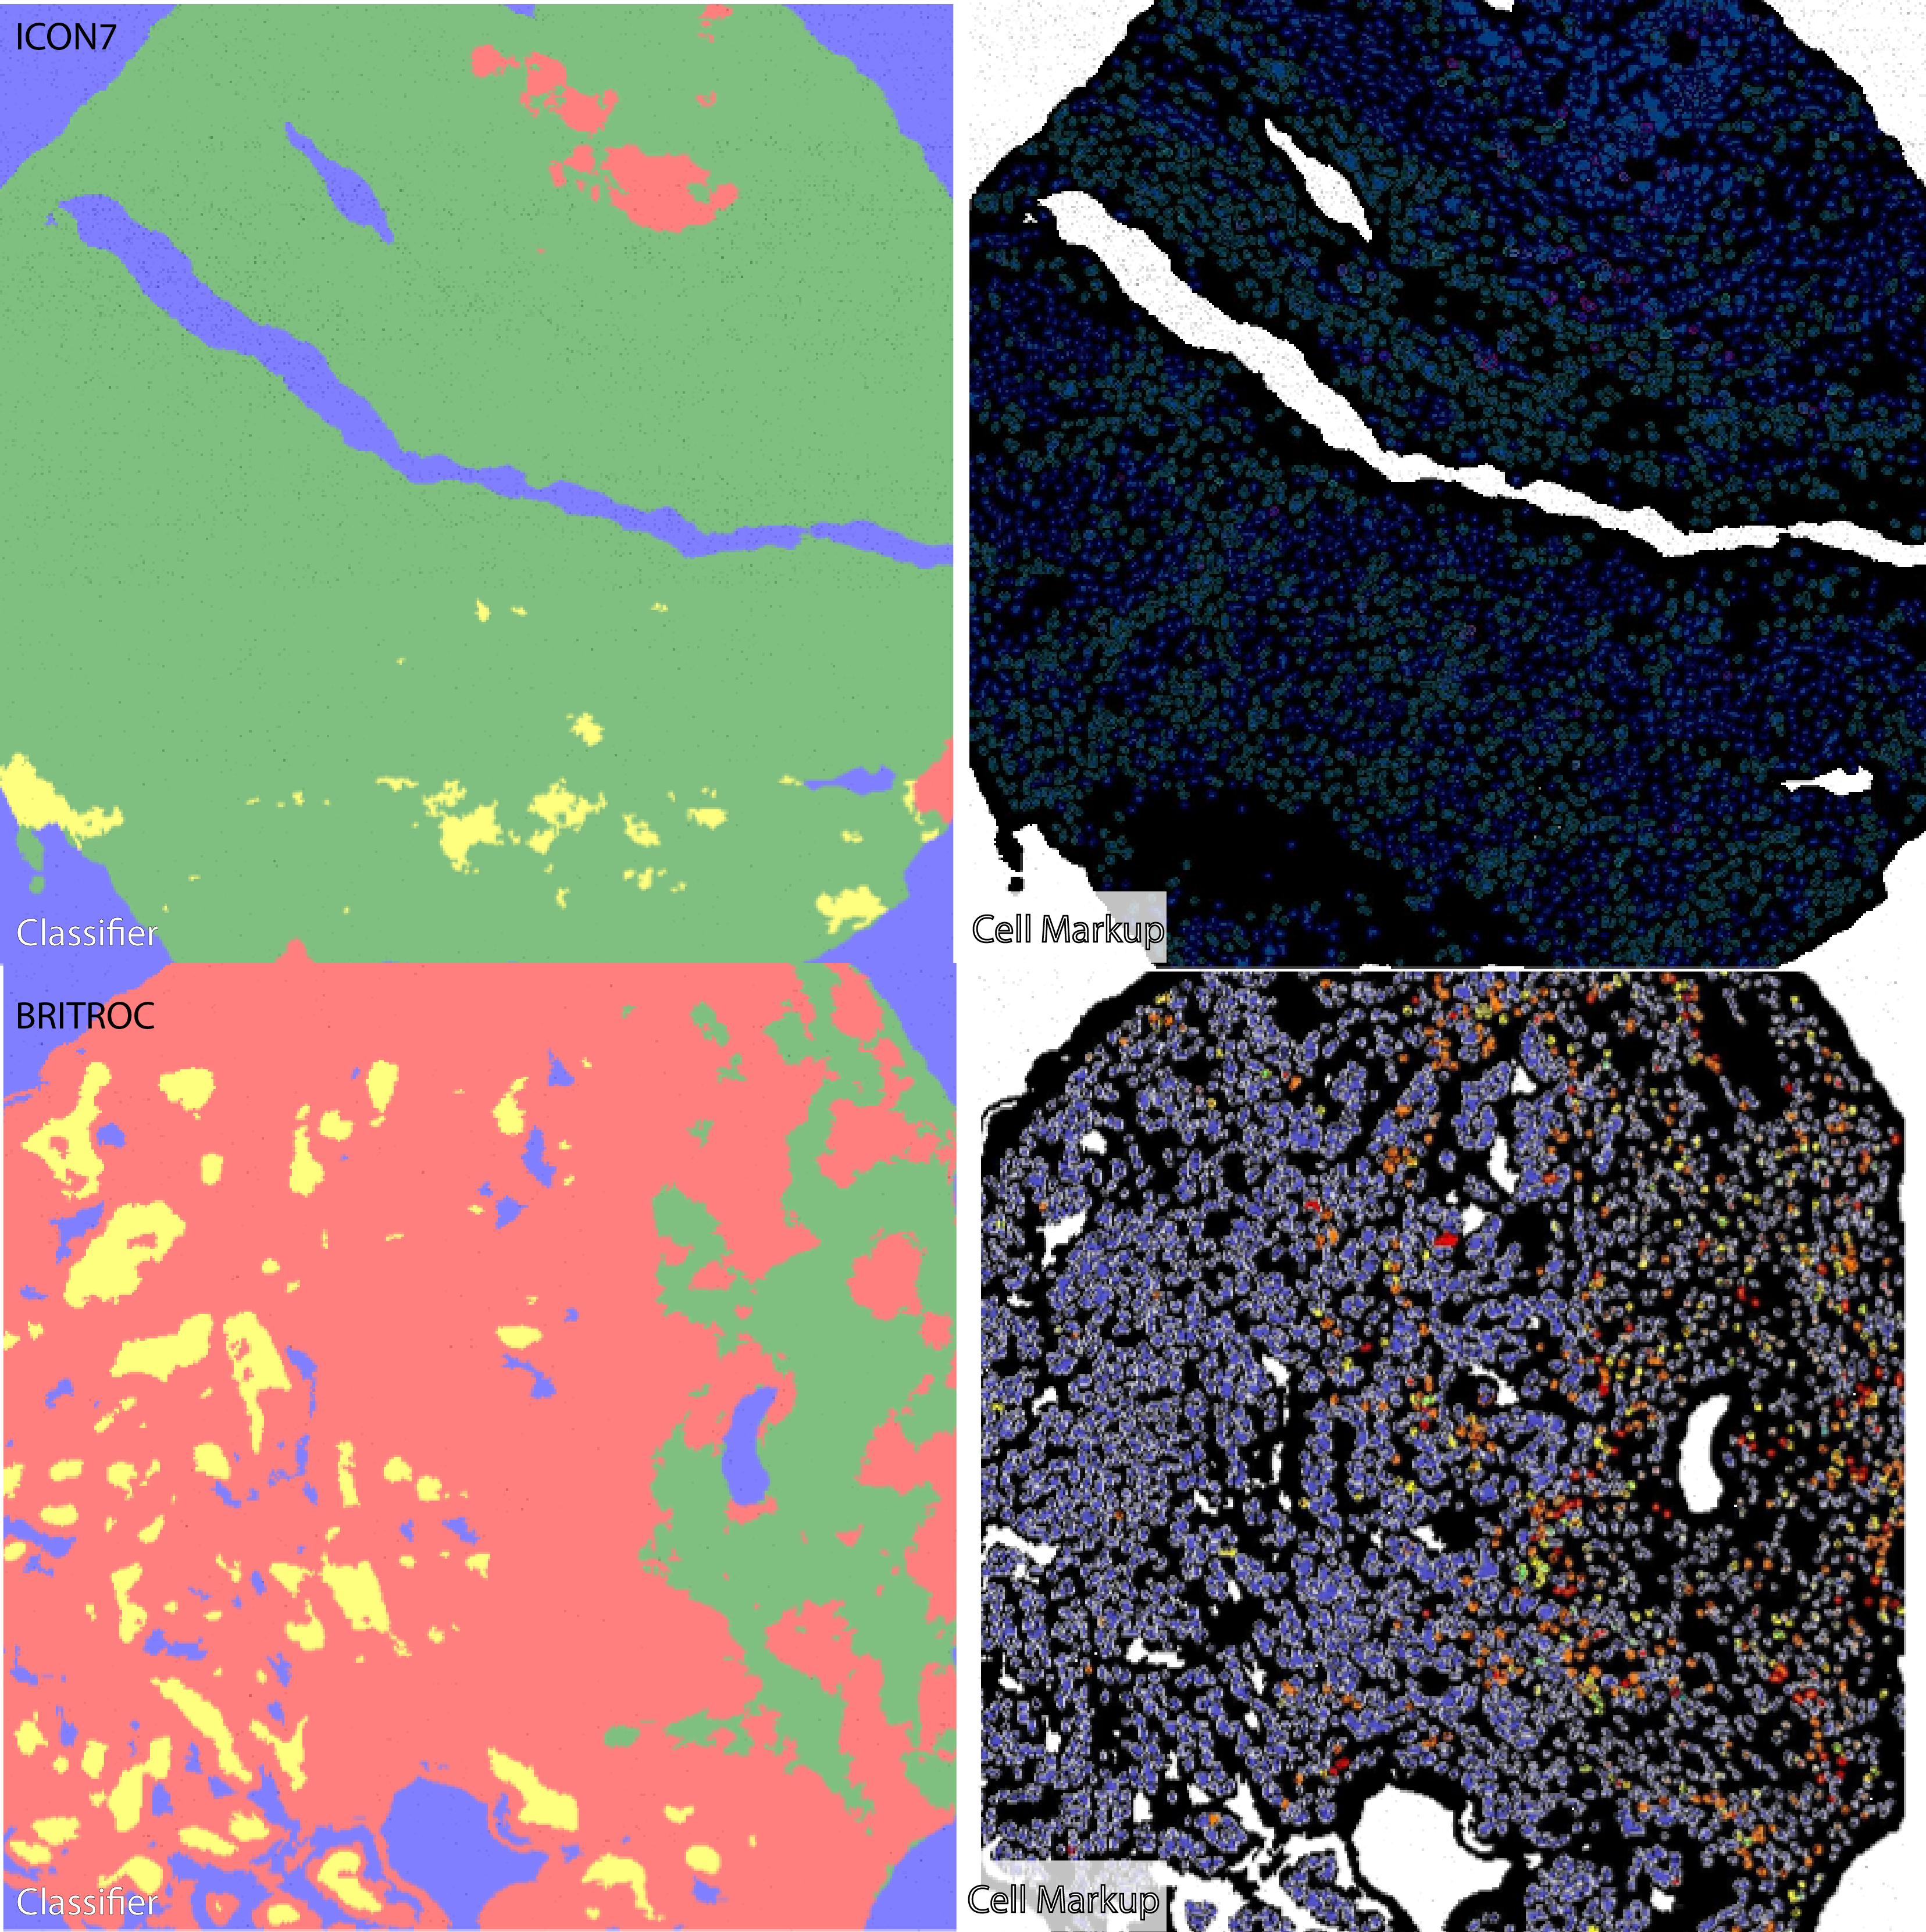
\includegraphics[width=0.5\textwidth]{Chapter4/figs/Thesis-09.png}
     \caption{Example of BRITROC and ICON7 classifier region and cell markup from HALO on IMC images.}
     \label{fig:IMC_example}
 \end{figure}
 
\subsubsection{IMC validation}

In order to validate the tissue and cell classification of the IMC, I used multiplexed IHC from serial sections of the same cohort to compare. Figure \ref{fig:IMC_IHC_corr} shows the correlation between IHC and IMC derived CD8/CD68 and between IMC and IHC derived stroma/tumour quantities.

\begin{figure}
    \centering
    \includegraphics{corr_IMC}
    \caption{Correlation between the epithelium quantity, CD8 cell density and CD68 cell density as measured in IHC and IMC on the BRITROC cohort.}
    \label{fig:IMC_IHC_corr}
\end{figure}

\subsection{Exploratory data analysis of TMA1}

The BRITROC cohort composed 3 TMAs in triplicate, I decided to use the first TMA in order to do an exploratory analysis for hypothesis generation. I would then be able to test the statistical significance of such hypotheses on both the other two TMAs and the ICON7 cohort. 

The first exploratory investigation of this dataset was to investigate the correlations between immune populations to validate the results found in earlier chapters and to build up a picture of which features of the micro-environment are connected.

I first investigated the correlation between numbers of CD3, CD8 and PD-1 positive cell areas in samples.

\begin{figure}
    \centering
    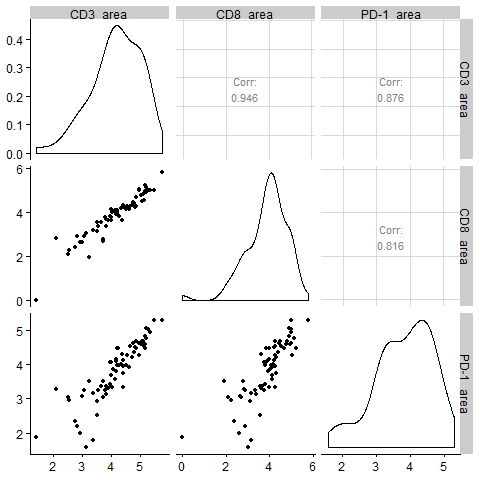
\includegraphics[width=0.5\textwidth]{Chapter4/figs/BRITROC_CD3_CD8_PD-1_corr.png}
    \caption{CD3, CD8, PD-1}
    \label{fig:CD8_CD3_PD1}
\end{figure}

\begin{figure}
    \centering
    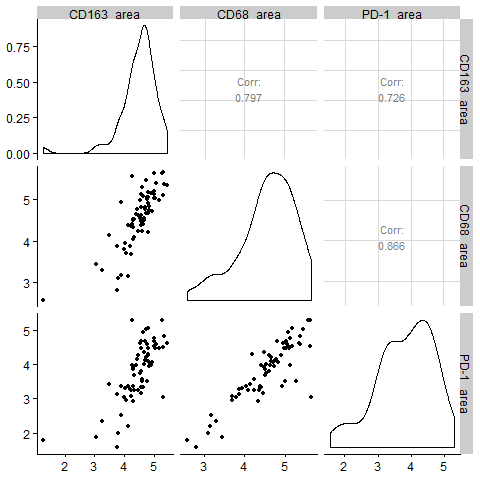
\includegraphics[width=0.5\textwidth]{Chapter4/figs/BRITROC_CD163_CD68_PD-1_corr.png}
    \caption{CD163, CD68, PD-1}
    \label{fig:CD163_CD8_PD1}
\end{figure}

\begin{figure}
    \centering
    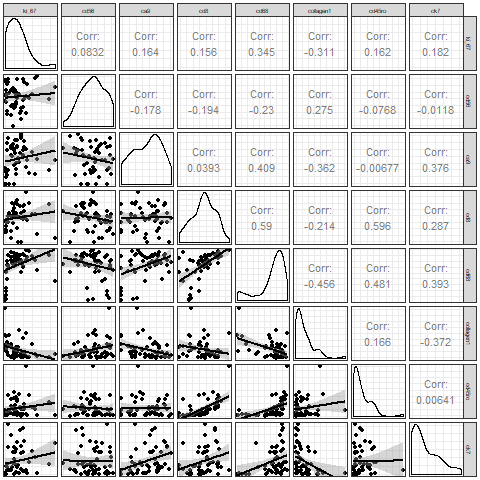
\includegraphics{Chapter4/figs/Britroc_cell_correlation2.png}
    \caption{Scatterplots of correlations between number of cells positive for each marker.}
    \label{fig:britroc_corr_scatt}
\end{figure}

\begin{figure}
    \centering
    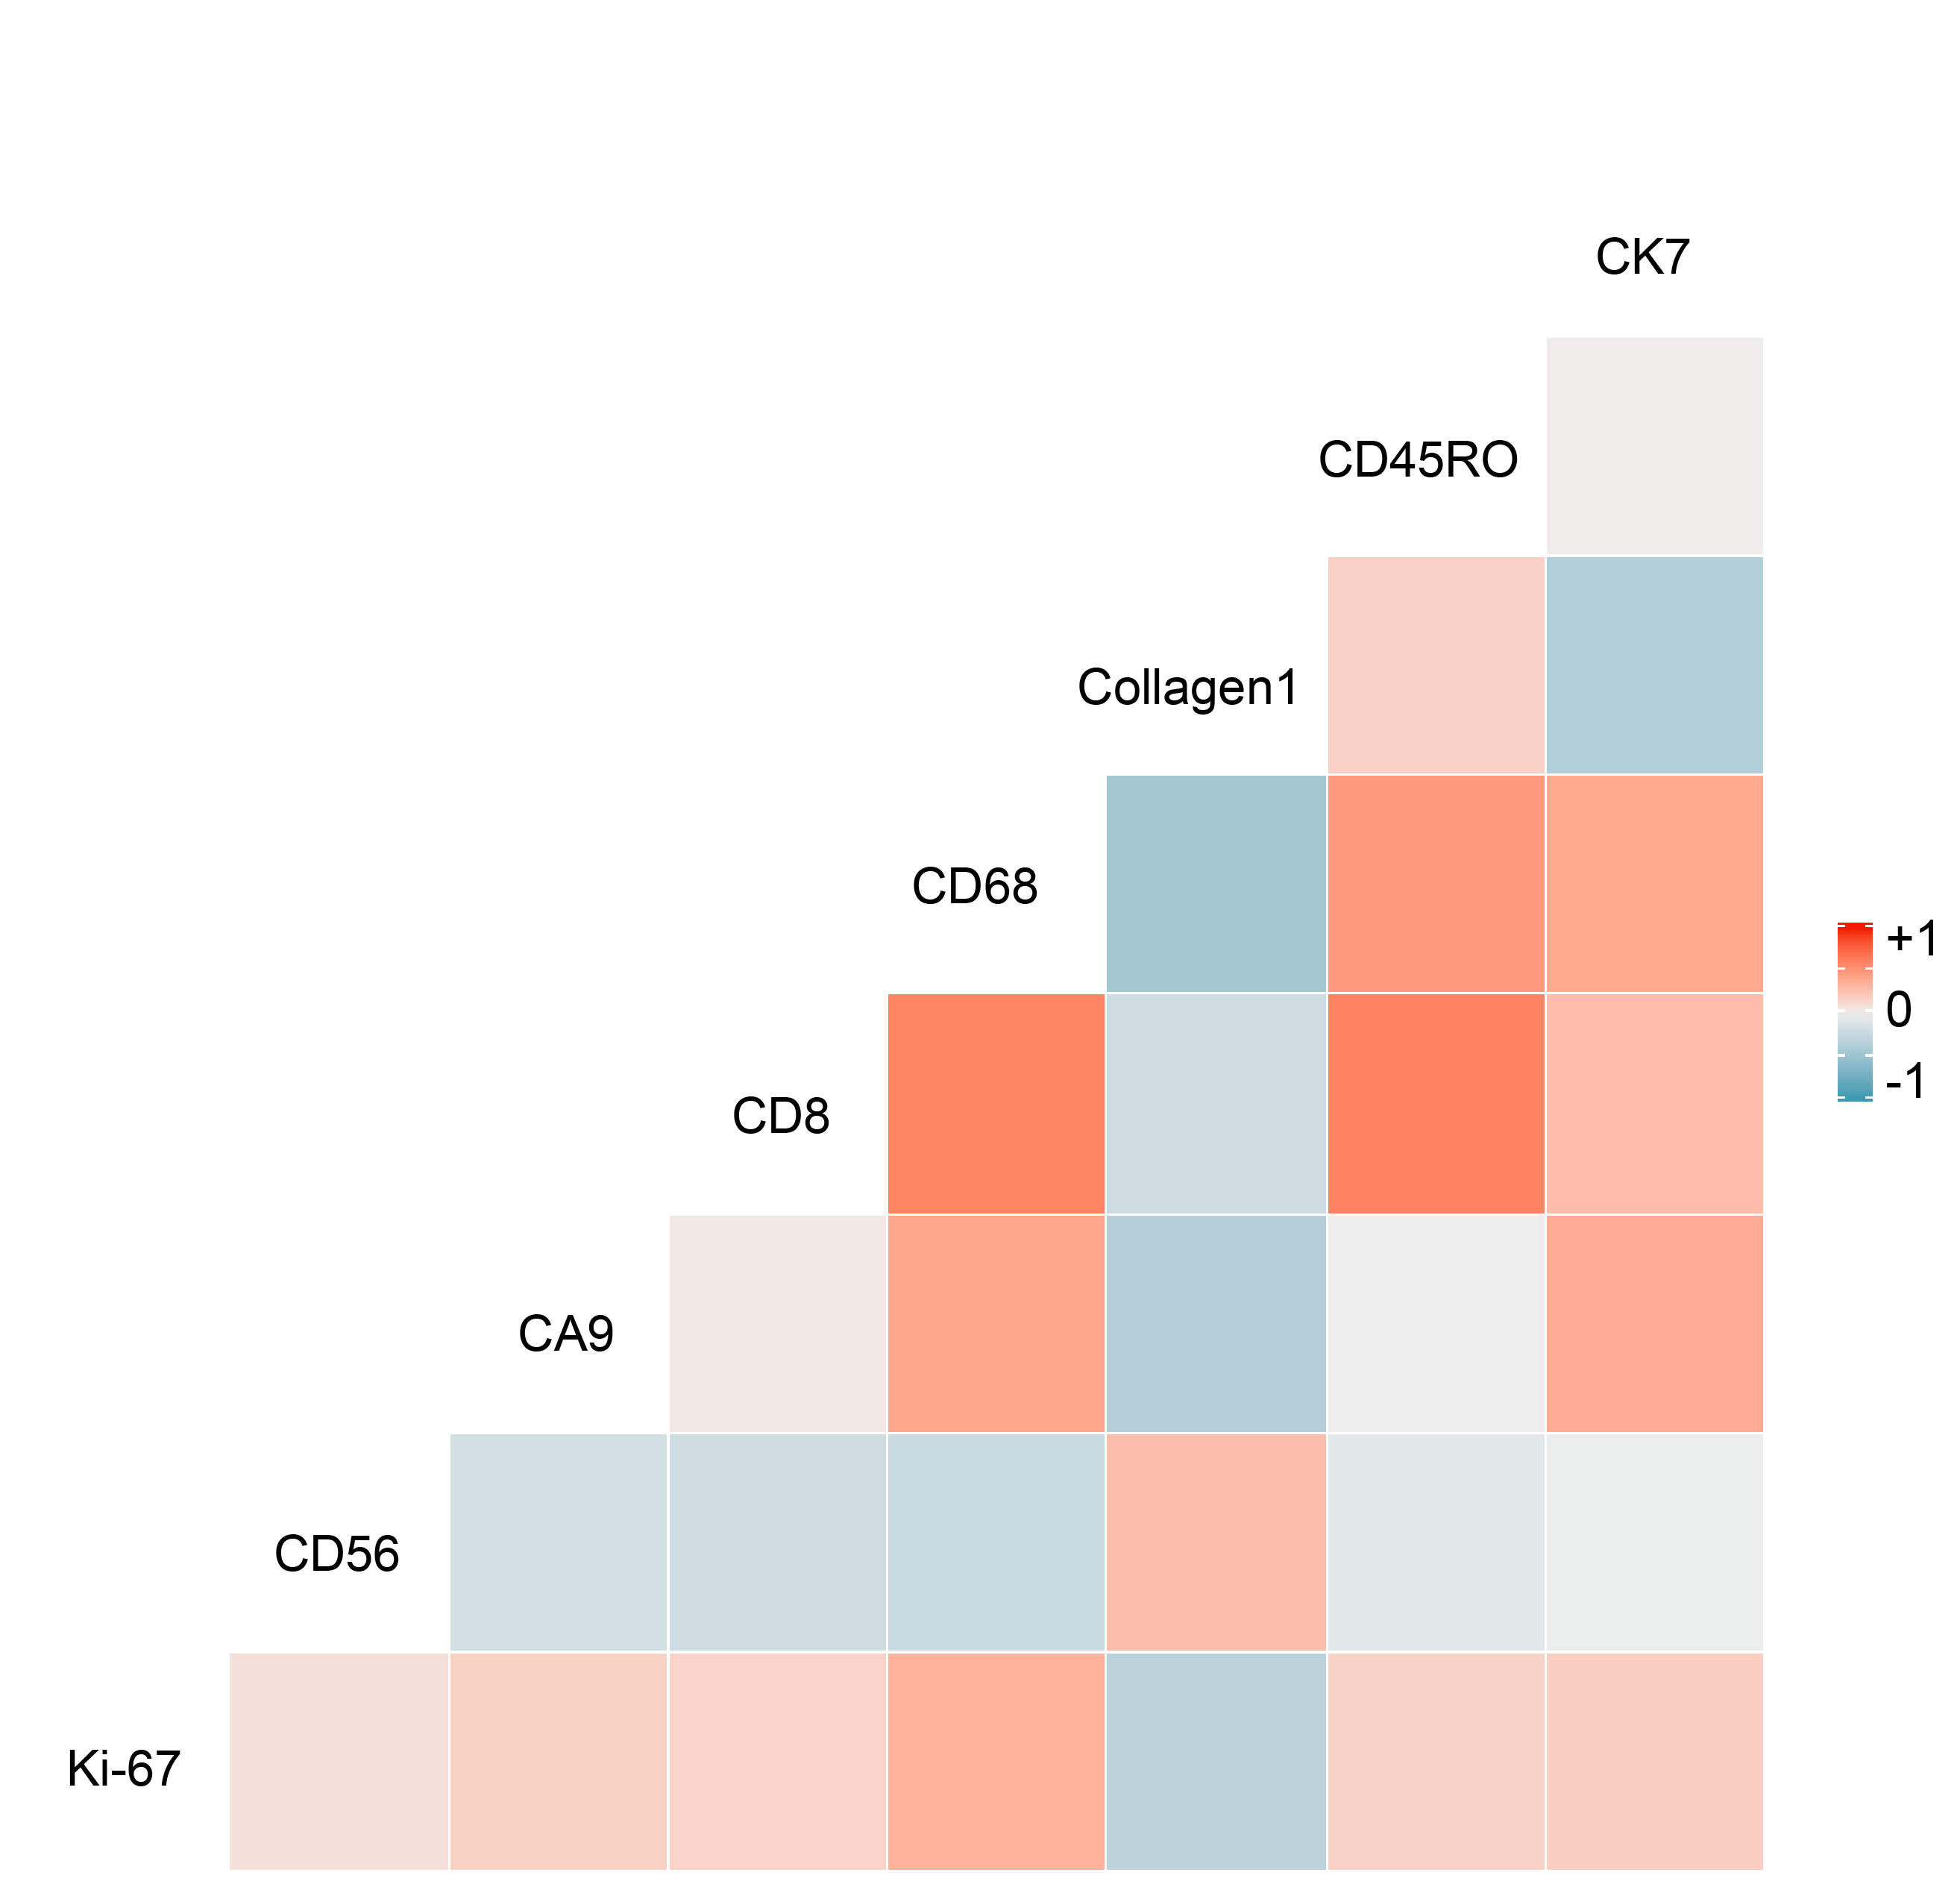
\includegraphics[width=0.5\textwidth]{Chapter2/Figs/Raster/correlation_britroc.png}
    \caption{Heatmap of correlations between number of cells positive for each marker.}
    \label{fig:britroc_corr_heat}
\end{figure}

Figures \ref{fig:britroc_corr_scatt} and \ref{fig:britroc_corr_heat} show the basic correlations between the number of CD8+, CD68+, CA9, CK7, Collagen1, CD45RO, CD56 and Ki-67+ cells in the BRITROC TMA. CD8, CD68 and CD45RO, the populations investigated in Chapter 1, show the strongest positive correlations. I also see the negative correlation we would expect between the number of Collagen and Cytokeratin positive cells as these cells are mutually exclusive and determine the majority of the structure of a tissue. Despite seeing a higher density of infiltrate in stromal regions in earlier chapters, we see a negative correlation between the number of collagen positive cells and the number of immune cells in these samples.


\subsection{Collagen deposition and hypoxia}
CA9 expression predominantly occurs in epithelial cells and given the negative correlation between epithelial cell quantity and collagen,  I normalised the CA9 positive cells as a percentage of total epithelial cells. 

I found no correlation between the percentage of epithelium positive for CA9 staining and the area Collagen weak or strong staining. 



\subsection{Principal Component Analysis}
In order to carry out a meaningful analysis across such a large number of measurements in multiple tissue regions, I used principal component analysis as in Chapter 2 in order to examine the patterns across the immune infiltrates. 

\subsection{Comparing immune cell densities between epithelium, high density and low density collagen}

\subsubsection{Macrophages}

CD68 and CD163 are both macrophage markers and macrophages are associated with collagen remodelling. I assessed the difference in the quantity of these macrophages across different strengths of collagen staining and the epithelium. I found no difference between the density of macrophage infiltration of collagen and epithelium.

\begin{figure}
    \centering
    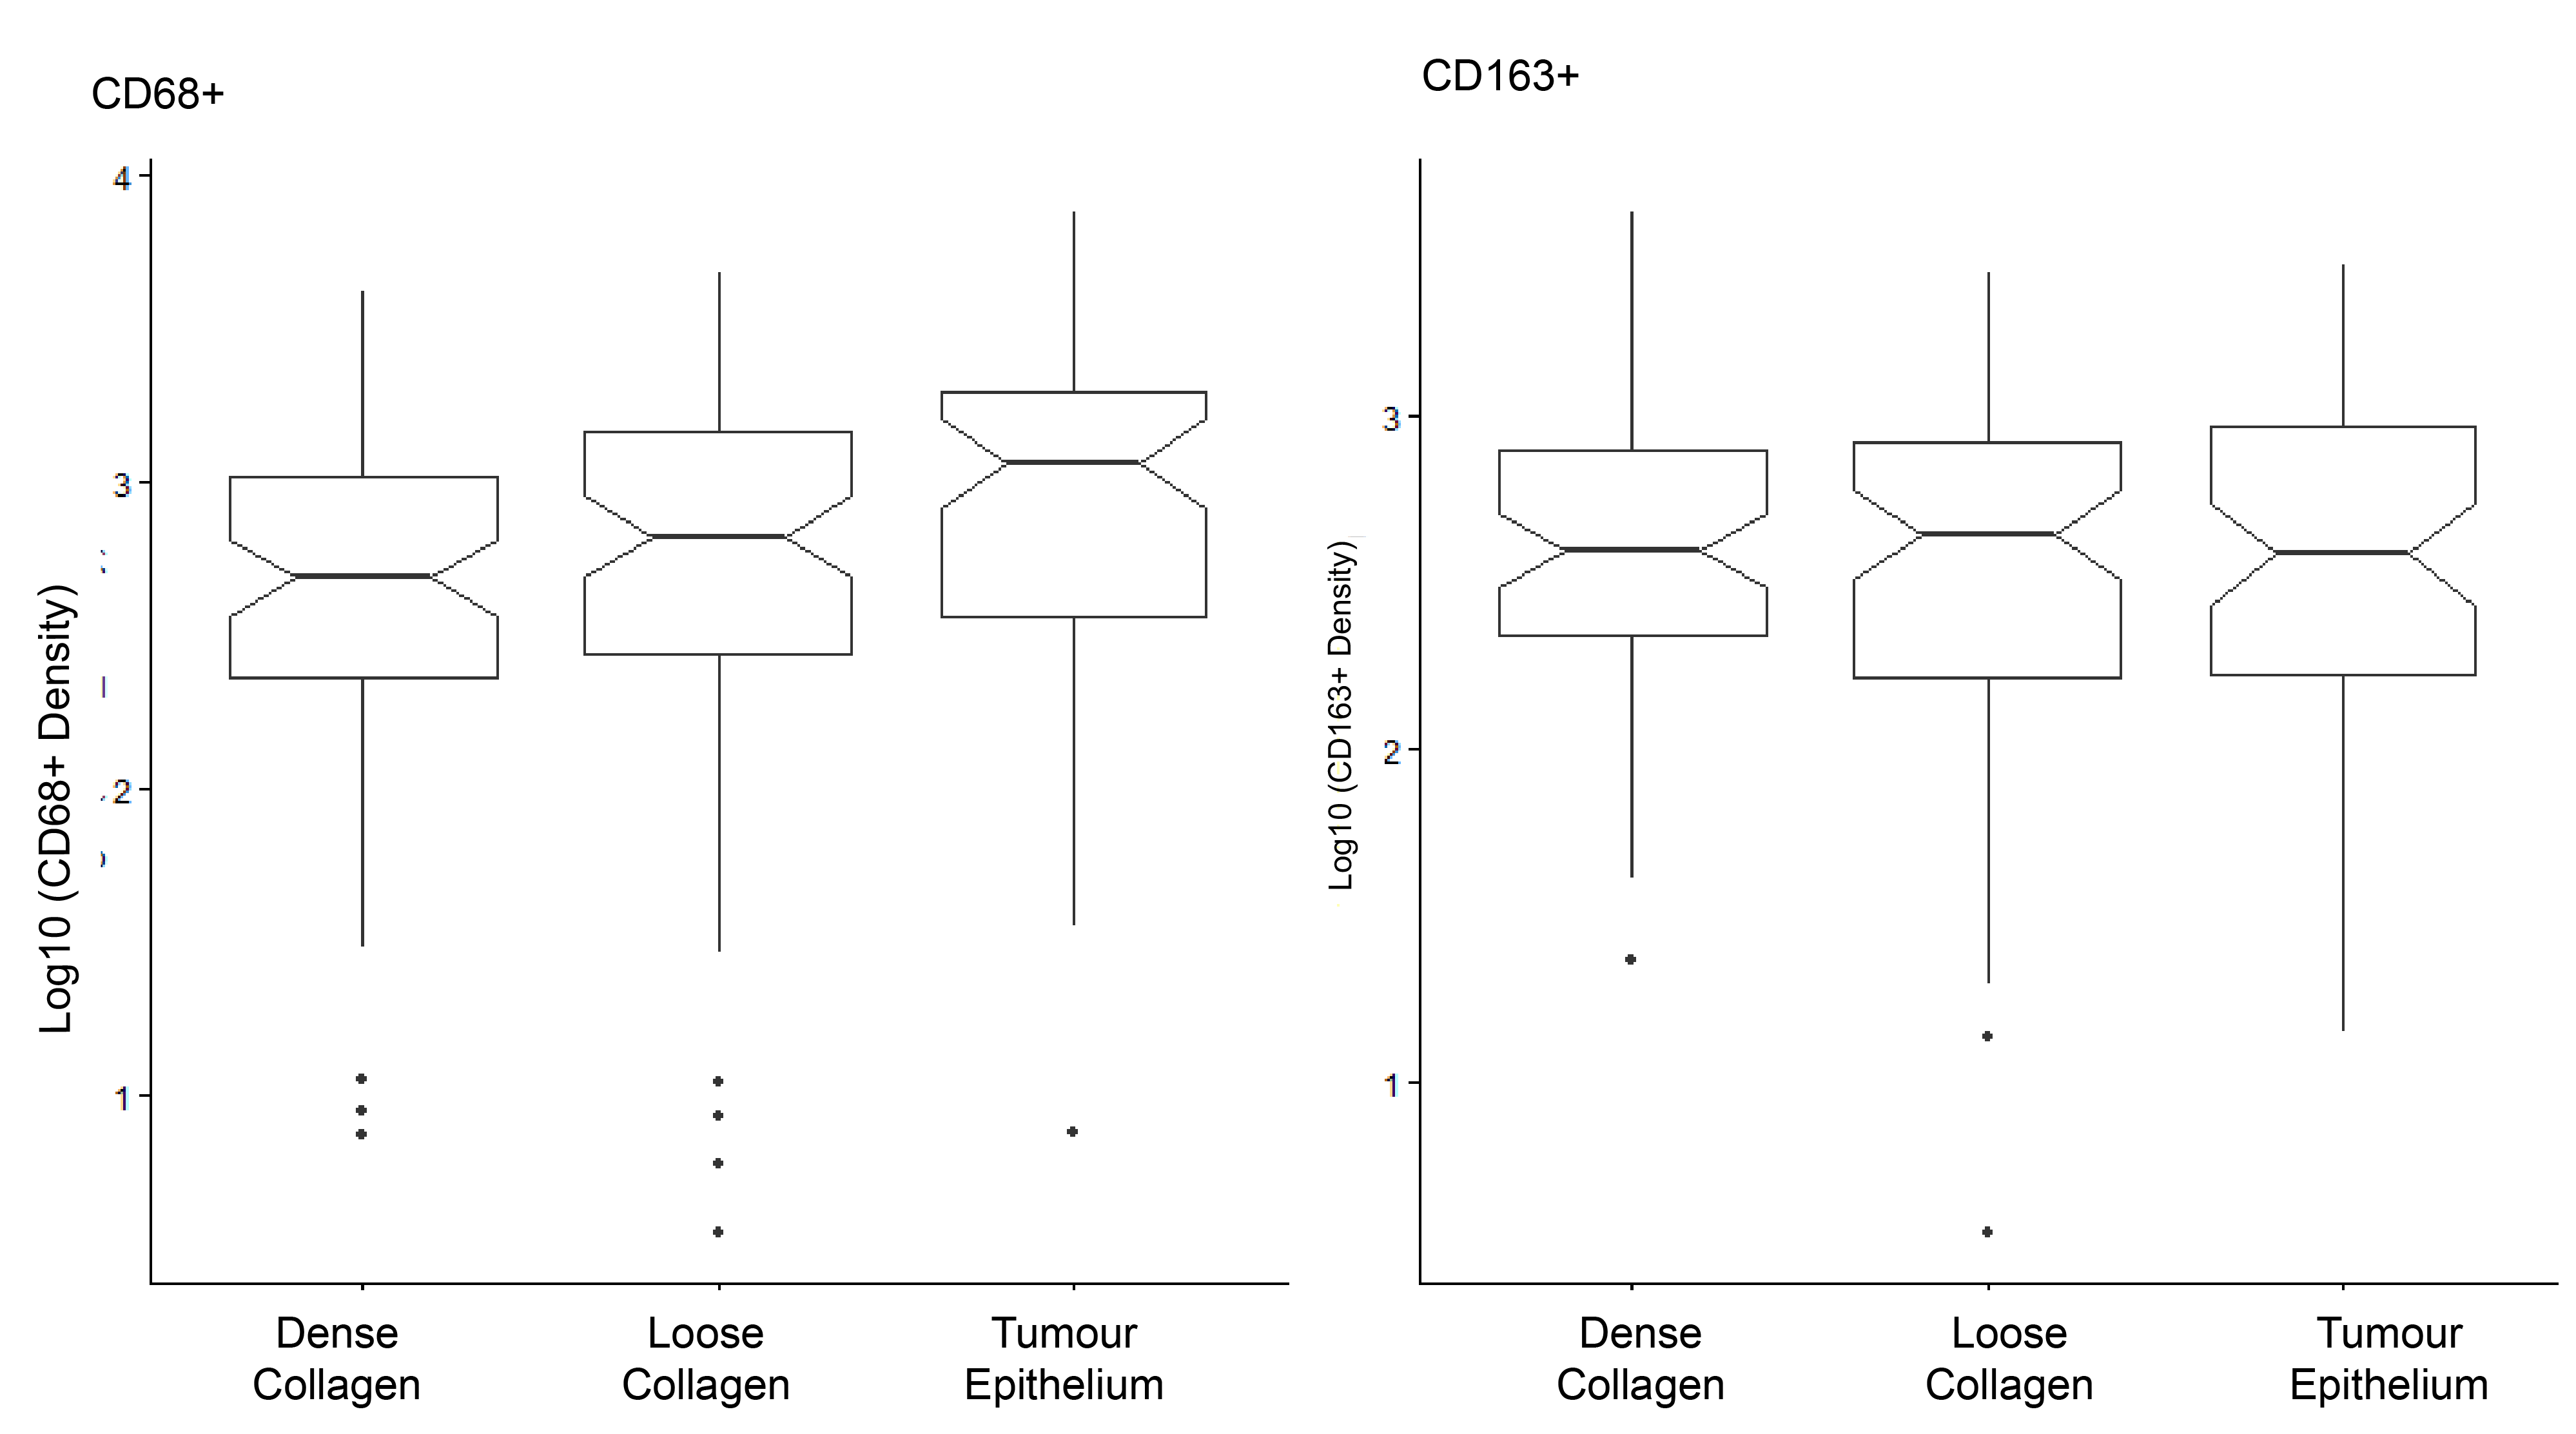
\includegraphics[width=0.9\textwidth]{Chapter4/figs/Thesis-10.png}
    \caption{Distribution of densities of CD68+ and CD163+ cells in the dense collagen, loose collagen and epithelial regions of the tumour section.}
    \label{fig:distribution}
\end{figure}

The area density of the immune infiltrates does not vary between, given that the nuclear 




\section{Discussion}
I utilised the multi-marker method of IMC on sections of tissue from BRITROC and ICON7. Investigating the relationship between infiltration of immune cells and the presence of hypoxia and structure.
